\graphicspath{{introduction/fig/}}

\chapter{Introduction}
\label{chap:introduction}
% TODO {introduction}
The prevalence of neural networks (NNs) has positioned them as a foundational technology in modern artificial intelligence. However, as their use has grown, so too has the focus on their inherent mechanistic limitations. Two of the most significant drawbacks of NNs are their lack of explainability---the "black-box" effect---and the immense computational cost required for training. A novel field, weight space learning, emerges as an exploration of these very challenges.


Weight space learning primarily focuses on developing methods to represent the numerical weights of NN models in a latent space, which can then be used for various downstream tasks. The field mainly considers two types of tasks: generative and discriminative.

In the discriminative application, models use the weights of already-trained models as input to accurately predict meta-information about the original model. For example, previous work has used [x method] to predict [y].

In the generataive application, x method was used by y, z did this etc. etc. 


The focus of this report is to extend the idea of laten weight representations, to a shared represeentation space. Where a model's weights, results and the dataset it was trained on are all represented in a shared space. Figure \ref{fig:pipeline} outlines the 

What the planned design is, and how it contriubutes to the problem outlines in par 1

    % TODO {outline_paragraph}
    In Section 1 we will discuss x, next y, concluded by z in attempt to showcase that this report is the best
    % TODO {outline_paragraph}

% TODO {introduction}


\begin{figure}[!t]
    \centering
    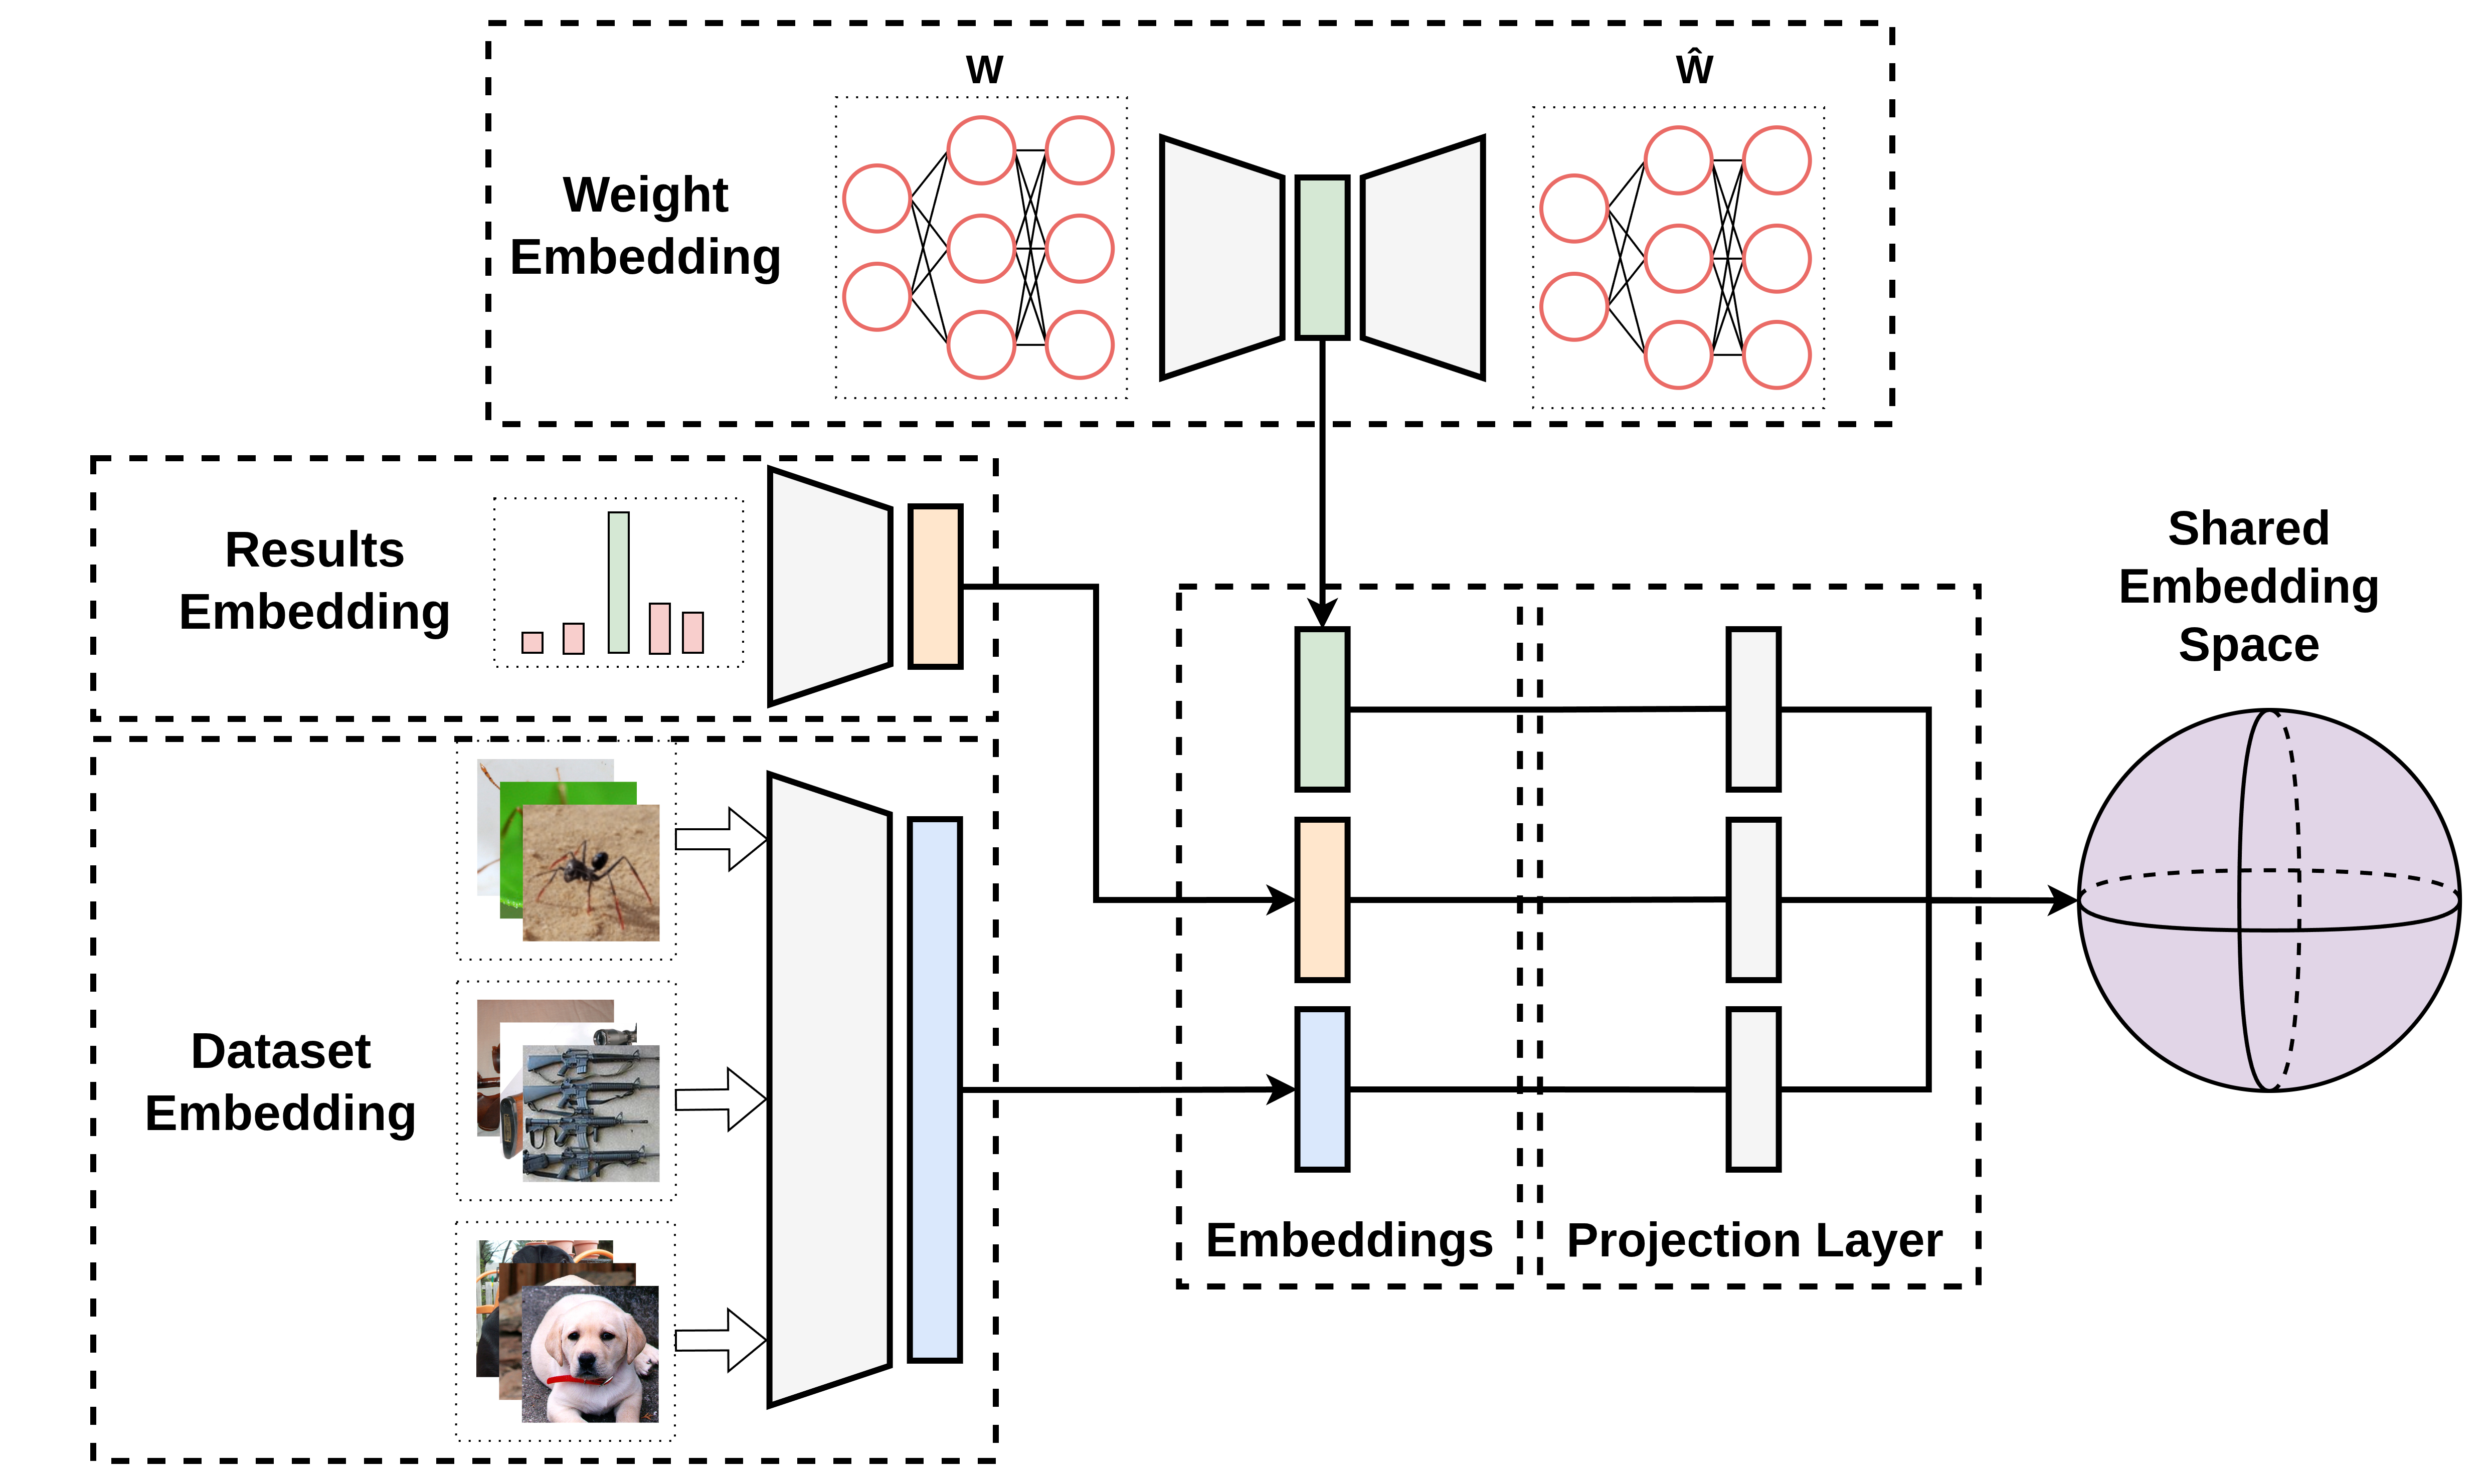
\includegraphics[width=0.75\linewidth]{pipeline.png}
    \caption[A figure illustrating the process of embedding a dataset,model weigths and results into a shared embedding space ]{A representation of the process of embedding a dataset, model weights and results in a shared embedding space. A dataset embedded using a pretained CLIP encoder, averaging over all images. Model weights embedded using a autoregressive encoder. Model results embeddings and the shared embedding space created through contrastive learning \cite{dahl+etal_taslp12}  }
    \label{fig:pipeline}
\end{figure}





% \section{Section heading}

% This is some section with two table in it: Table~\ref{tbl:exemplars} and Table~\ref{tbl:abx_speaker}.

% \begin{table}[!h]
%     \mytable
%     \caption{Performance of the unconstrained segmental Bayesian model on TIDigits1 over iterations in which the reference set is refined.}
%     \begin{tabularx}{\linewidth}{@{}lCCCCC@{}}
%         \toprule
%         Metric     & 1 & 2 & 3 & 4 & 5 \\
%         \midrule
%         WER (\%)                        & $35.4$ & $23.5$ & $21.5$ & $21.2$ & $22.9$ \\
%         Average cluster purity (\%)       & $86.5$ & $89.7$ & $89.2$ & $88.5$ & $86.6$ \\
%         Word boundary $F$-score (\%)         & $70.6$ & $72.2$ & $71.8$ & $70.9$ & $69.4$ \\
%         Clusters covering 90\% of data   & 20             & 13 & 13 & 13 & 13 \\
%         \bottomrule
%     \end{tabularx}
%     \label{tbl:exemplars}
% \end{table}


% \begin{table}[!h]
%     \renewcommand{\arraystretch}{1.1}
%     \centering
%     \caption{A table with an example of using multiple columns.}
%     \begin{tabularx}{0.65\linewidth}{@{}lCCr@{}}
%         \toprule
%         & \multicolumn{2}{c}{Accuracy (\%)} \\
%         \cmidrule(lr){2-3}
%         Model    & Intermediate & Output & Bitrate\\
%         \midrule
%         Baseline & 27.5         & 26.4   & 116 \\
%         VQ-VAE   & 26.0         & 22.1   & 190 \\
%         CatVAE   & 28.7         & 24.3   & 215 \\
%         \bottomrule
%     \end{tabularx}
%     \label{tbl:abx_speaker}
% \end{table}

% \newpage

% This is a new page, showing what the page headings looks like, and showing how to refer to a figure like Figure~\ref{fig:cae_siamese}.

% \begin{figure}[!t]
%     \centering
% %     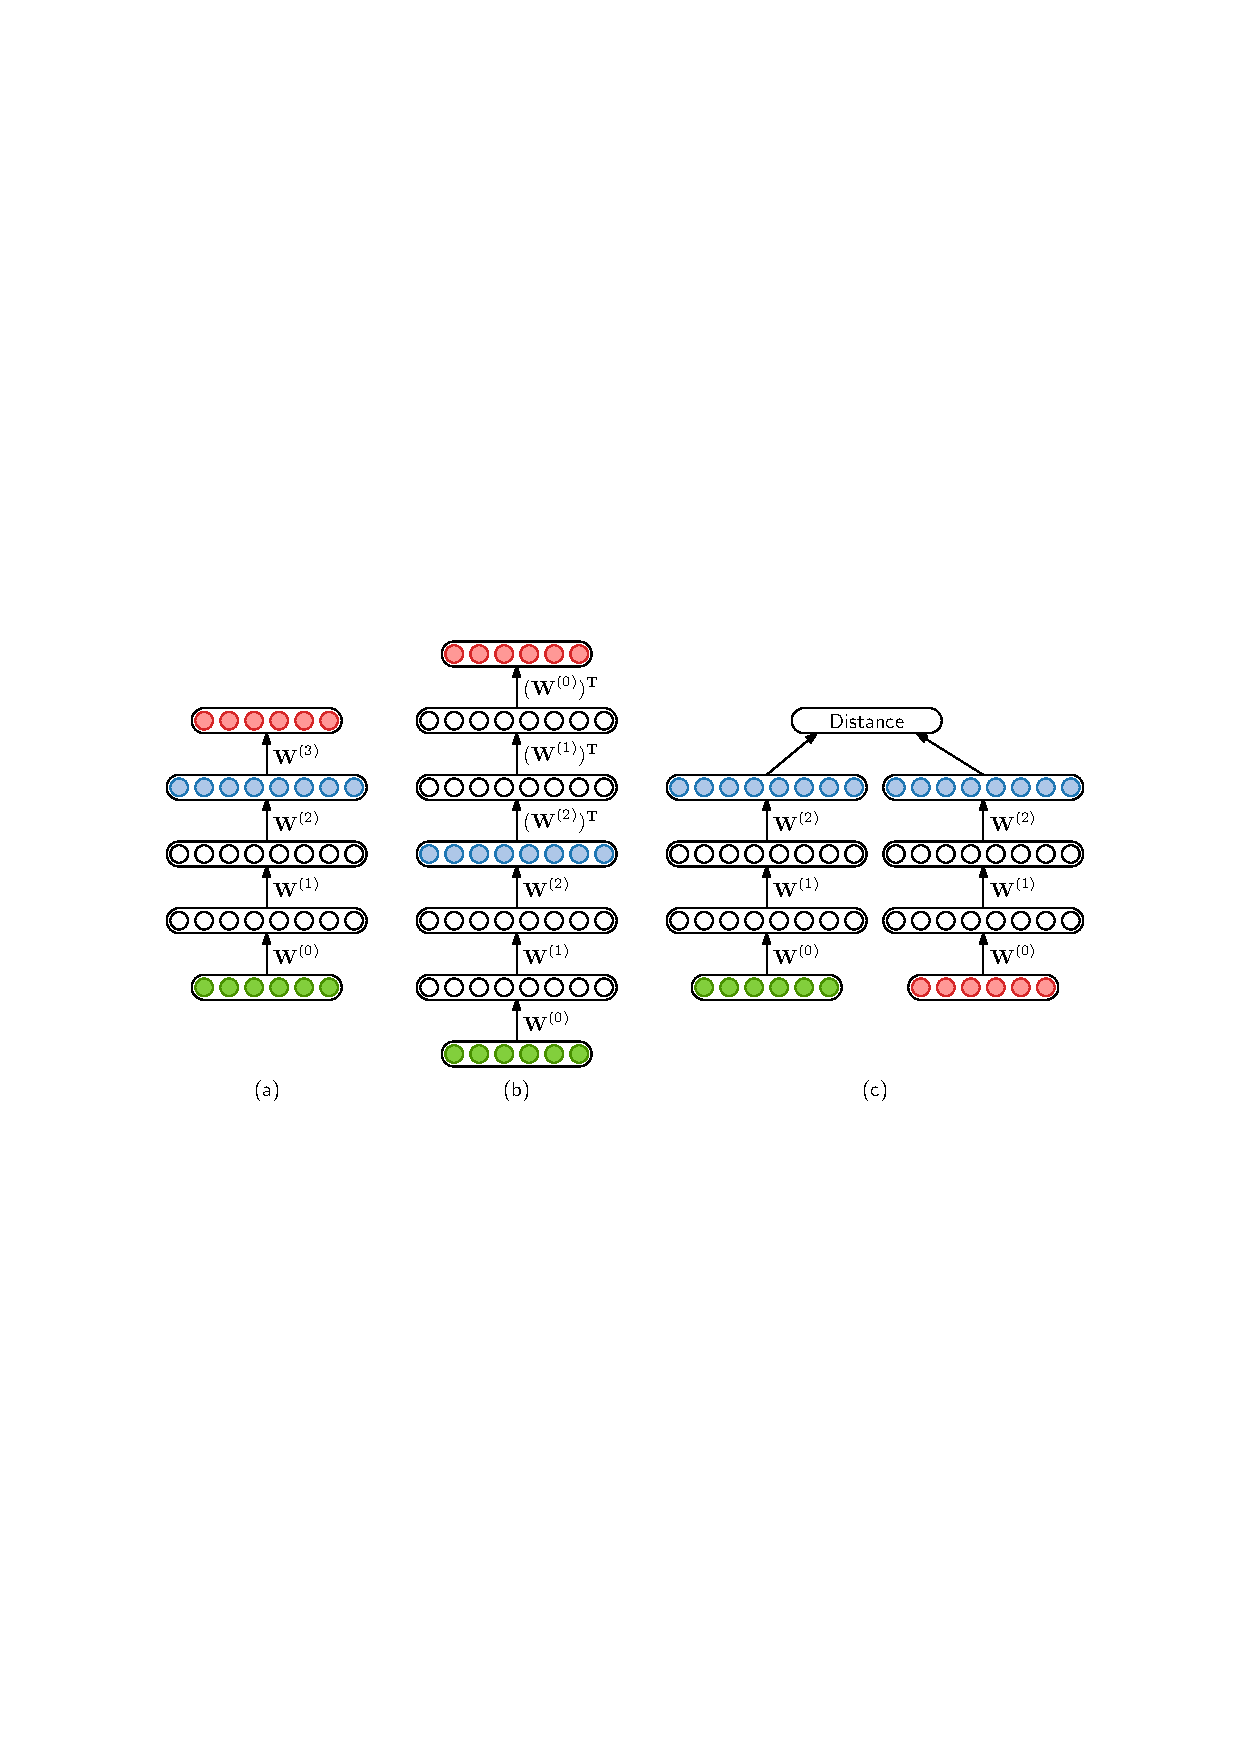
\includegraphics[width=\linewidth]{cae_siamese}
%     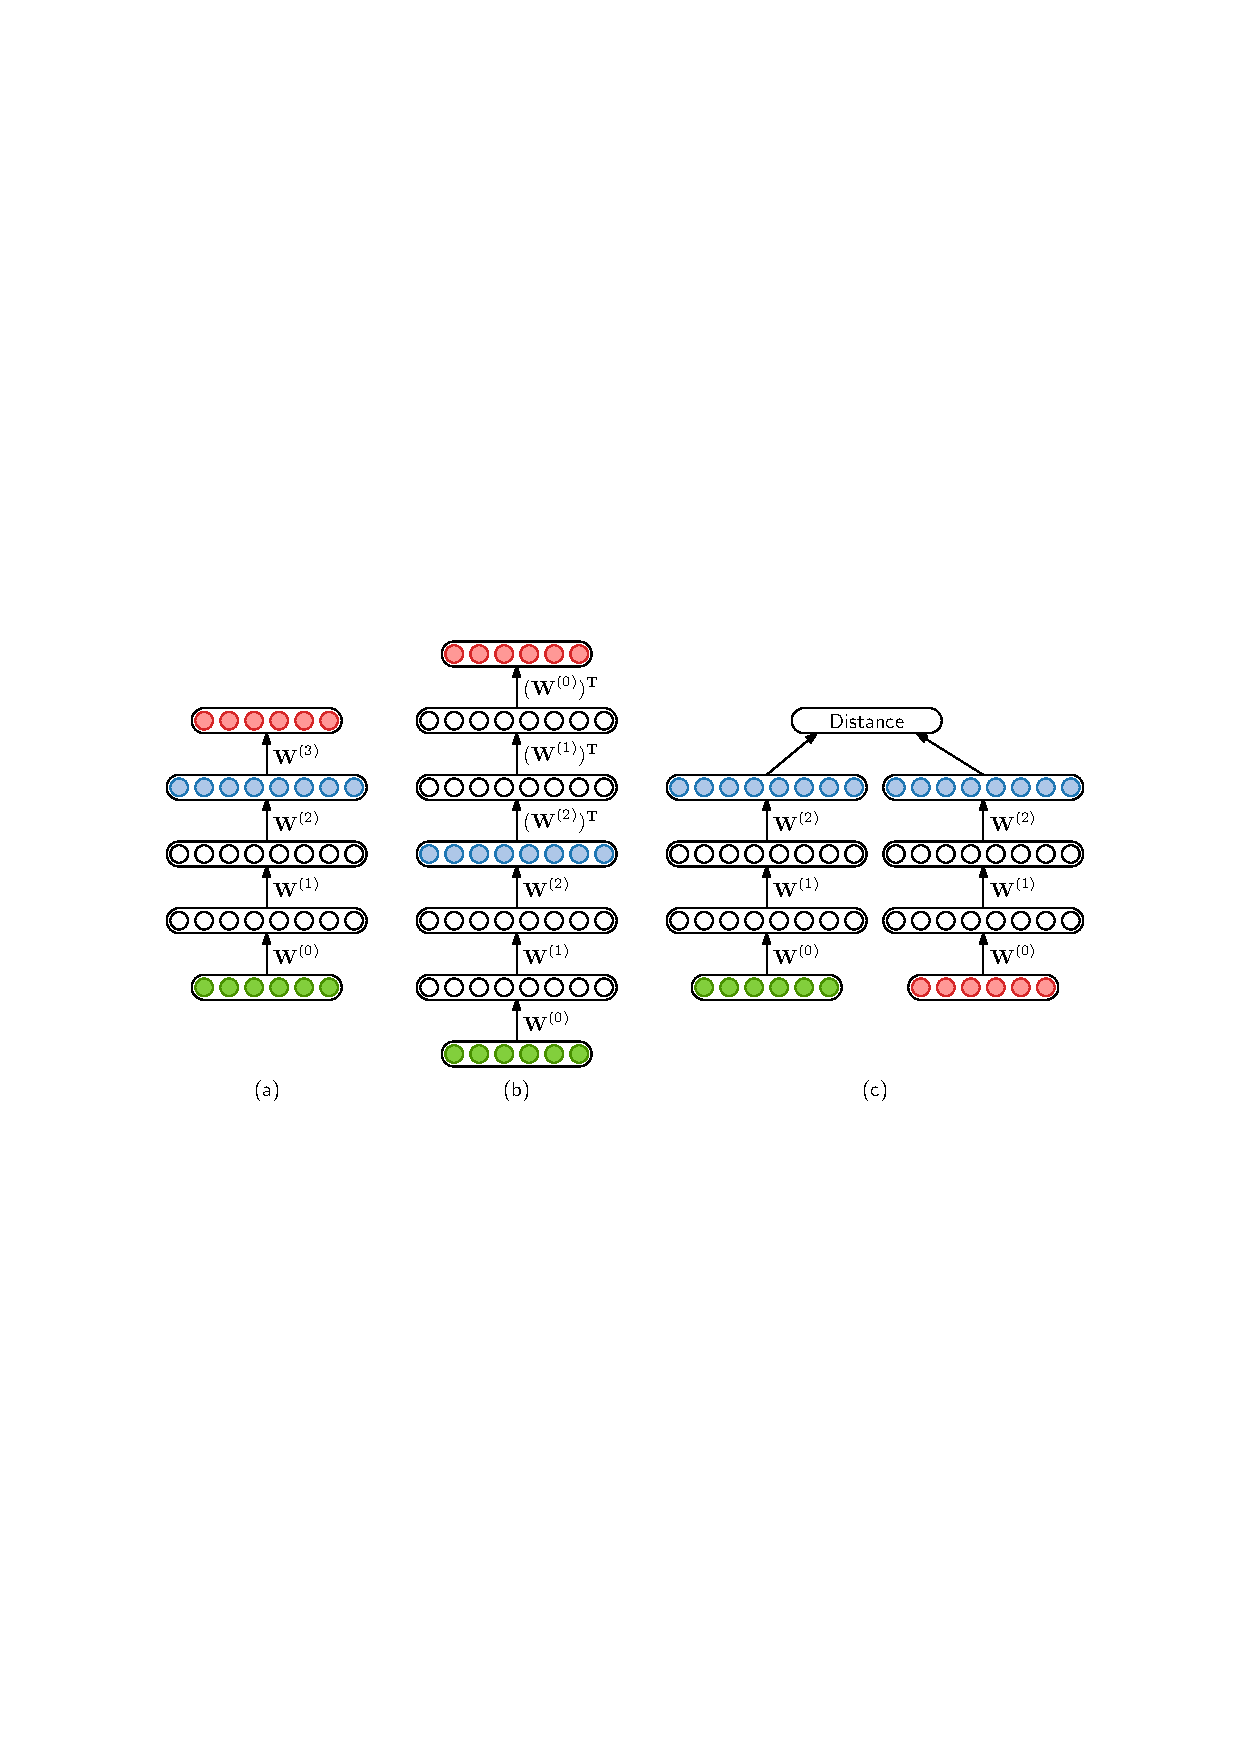
\includegraphics[width=0.918\linewidth]{cae_siamese}
%     \caption[I am the short caption that appears in the list of figures, without references.]{
%     (a) The cAE as used in this chapter. The encoding layer (blue) is chosen based on performance on a development set.
%     (b) The cAE with symmetrical tied weights. The encoding from the middle layer (blue) is always used.
%     (c) The siamese DNN. The cosine distance between aligned frames (green and red) is either minimized or maximized depending on whether the frames belong to the same (discovered) word or not.
%     A cAE can be seen as a type of DNN~\cite{dahl+etal_taslp12}.
%     }
%     \label{fig:cae_siamese}
% \end{figure}


% The following is an example of an equation:
% \begin{equation}
% P(\vec{z} | \vec{\alpha}) = \int_{\vec{\pi}} P(\vec{z} | \vec{\pi}) \, p(\vec{\pi} | \vec{\alpha}) \, \textrm{d} \vec{\pi}
% = \int_{\vec{\pi}} \prod_{k = 1}^K \pi_k^{N_k} \frac{1}{B(\vec{\alpha})} \prod_{k = 1}^K \pi_k^{\alpha_k - 1} \, \textrm{d} \vec{\pi}
% \label{eq:example_equation}
% \end{equation}
% which you can subsequently refer to as~\eqref{eq:example_equation} or Equation~\ref{eq:example_equation}.
% But make sure to consistently use the one or the other (and not mix the two ways of referring to equations).


